\vspace{-10px}%
\section{Related Work}\label{sect:related}
\vspace{-4px}
\subsection{Data parallel training}\label{sect:related_data_parallel}
\vspace{-4px}

The most popular way to accelerate neural network training with multiple devices is data-parallel training~\cite{valiant1990bridging,goyal2017accurate,You2020Large}. On each optimization step, this strategy splits the training batch among participants. Each participant then runs forward and backward passes to obtain gradients of the objective function on their part of the training batch. After that, we can aggregate the gradients from workers and perform an optimization step. There are two main strategies for this aggregation.

Historically, the first solution to gradient aggregation was to use Parameter Server (PS)~\cite{parameter_server_first}: a separate process or a dedicated server that keeps track of model parameters and optimizer statistics. After each round, the PS accumulates the gradients from each worker and updates the model parameters using SGD or any other optimizer, such as Adam~\cite{adam}. Finally, the server distributes the updated model parameters to workers.

This strategy is robust and easy to implement, but it requires the server to regularly download full model gradients from every single worker. As a result, the parameter server can quickly become a bottleneck for large-scale training~\cite{survey_distributed2}\nocite{survey_distributed}. Since the original PS, researchers have proposed several modifications that reduce the communication load: accumulating multiple batches~\cite{localsgd_first}, compression~\cite{lin2018deep,pmlr-v97-koloskova19a}, server sharding~\cite{sharded_ps_first,byteps}. A more detailed overview is given in Appendix~\ref{sect:post_related}.

In turn, many practical distributed training systems have instead switched to averaging with All-Reduce ~\cite{goyal2017accurate,mikami2019massively,shoeybi2019megatron,You2020Large}. This name refers to a collection of protocols originally developed for HPC applications. Workers can follow these protocols to collectively compute the average\footnote{All-Reduce works with any commutative associative operation, such as min, max, or product.} gradient more efficiently than with a central server.

\subsection{Communication-efficient All-Reduce}\label{sect:related_allreduce}
There are several all-reduce protocols optimized for different network topologies. The simplest one is known as Butterfly All-Reduce~\cite{bandwidth_optimal_allreduce}. Each of $N$ participants splits its local vector into $N$ chunks. Then, $i$-th worker aggregates $i$-th chunk of data from all peers and sends back the averaged chunk.

\begin{figure}[h!]
    \centering
    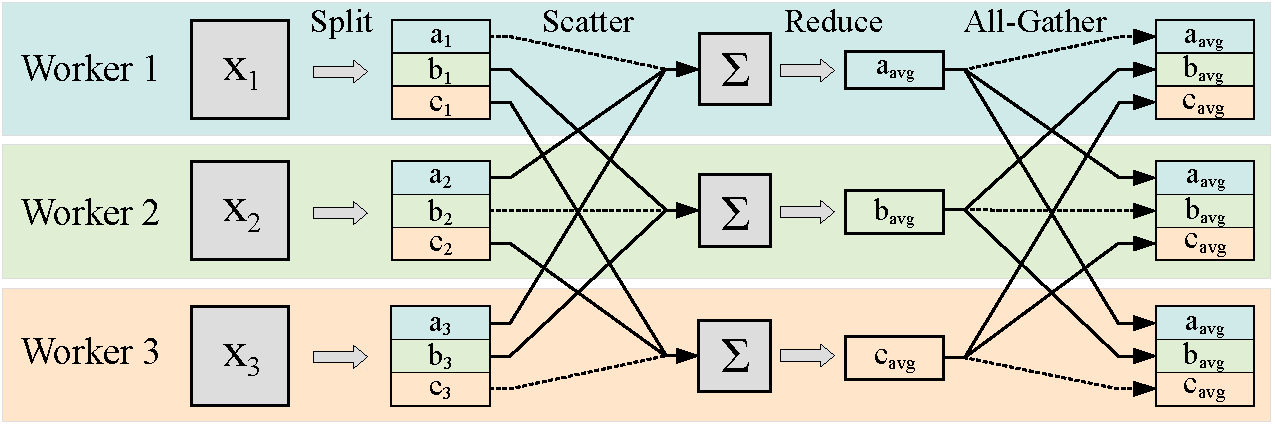
\includegraphics[width=0.65\linewidth]{resources/butterfly.pdf}
    \caption{A schematic illustration of Butterfly All-Reduce.}
    \label{fig:butterfly_allreduce}
\end{figure}

As long as the vector size $s$ is greater than $N$, this protocol uses $\cO\left(s \times \frac{N - 1}{N}\right)$ total bandwidth on each worker. However, it requires all-to-all communication, which is not always practical for the HPC infrastructure due to network contention~\cite{bandwidth_optimal_allreduce}. As a result, real-world systems typically use Ring or Tree All-Reduce, where each worker only communicates with a small subset of its peers.

These protocols enable highly efficient and scalable averaging with $\cO(1)$ or $\cO(\log N)$ total communication per worker, but they also share a common drawback: they cannot tolerate node failures or network instability. If any single participant fails to execute its part or takes long to respond, this paralyzes all other workers.

\subsection{Distributed training in unstable conditions}\label{sect:related_unreliable}
Some distributed training applications must deal with unstable network bandwidth and/or unreliable workers. This issue is most prevalent in federated learning~\cite{mcmahan2017communication,secure_aggregation,federatedlearningatscale}. When dealing with privacy-sensitive data distributed across multiple actors, such as hospital servers~\cite{fed_intel,fed_nvidia} or mobile phones~\cite{fed_google1,fed_google2}, one must train the model using whichever hardware and network available to those actors.

Another important motivational factor is cost: HPC-grade infrastructure can be prohibitively expensive, pushing researchers and practitioners towards commodity servers or preemptible cloud VMs that are significantly cheaper (see Appendix~\ref{sect:cloud_costs}). Another solution is to use volunteer computing~\cite{volunteer_dl_async, learning_at_home} with abundant, but even less reliable, compute resources.

Training under these conditions requires specialized strategies. At a small scale, one can deploy one or a few reliable parameter servers to aggregate the updates from workers. This strategy can tolerate individual node failures~\cite{proteus}, but scales poorly due to the reasons discussed in Section~\ref{sect:related_data_parallel}.

\subsection{Decentralized training}\label{sect:related_decentralized_training}
If there are too many participants for PS, it can be advantageous to use decentralized SGD via \textbf{gossip-based} averaging \cite{boyd2006randomized,tsitsiklis1984problems,lian2017can}. In this scenario, participants form a sparse graph: each worker periodically downloads parameters from its neighbors and mixes them with local parameters.

In essence, gossip-based averaging removes the communication bottlenecks of PS at the cost of using different local parameters on each peer. That said, gossip-based optimization algorithms can match, and sometimes even outperform, their centralized counterparts in terms of training speed~\cite{scaman2017optimal,scaman2018optimal,scaman2019optimal,lian2017can,assran2019stochastic}. However, the convergence properties of gossip averaging and gossip-based optimization methods significantly depend on the communication graph through the spectral properties of the mixing matrix~\cite{xiao2004fast,scaman2019optimal} or the Laplacian matrix of the network~\cite{merris1994laplacian,uribe2020dual}. 

Consequently, as the number of peers increases, gossip-based averaging has to either increase the number of neighbors (hence more communication) or accept slower convergence speed. Because of this, gossip is less communication-efficient than all-reduce algorithms reviewed in Section~\ref{sect:related_allreduce}. However, gossip-based algorithms are more robust to changes, which makes them applicable to time-varying networks~\cite{nedic2014distributed,nedic2016stochastic,nedic2018network,rogozin2019projected} and federated learning~\cite{ram2009asynchronous,yan2012distributed,yuan2016convergence}.

